\documentclass[Master,MSE,german]{twbook}
\usepackage[utf8]{inputenc}
\usepackage[T1]{fontenc}
\newcommand{\FHTWCitationType}{IEEE}
\usepackage{bibgerm}

% Definition Code-Listings Formatierung:
\usepackage[final]{listings}
\lstset{captionpos=b, numberbychapter=false,caption=\lstname,frame=single, numbers=left, stepnumber=1, numbersep=2pt, xleftmargin=15pt, framexleftmargin=15pt, numberstyle=\tiny, tabsize=3, columns=fixed, basicstyle={\fontfamily{pcr}\selectfont\footnotesize}, keywordstyle=\bfseries, commentstyle={\color[gray]{0.33}\itshape}, stringstyle=\color[gray]{0.25}, breaklines, breakatwhitespace, breakautoindent}
\lstloadlanguages{[ANSI]C, C++, [gnu]make, gnuplot, Matlab}

\makeatletter
\renewcommand\lstlistingname{Quellcode}
\renewcommand\lstlistlistingname{Quellcodeverzeichnis}

% Definition des Macros listoflolentryname analog zu listoflofentryname und listoflotentryname der KOMA-Klasse
\newcommand\listoflolentryname\lstlistingname
% Neudefinition der Zeilen des Quellcodeverzeichnisses wenn die Option listof=entryprefix gewählt wurde
\@ifclasswith{scrbook}{listof=entryprefix}
{%
    \renewcommand\l@lstlisting[2]{\@dottedtocline{1}{1.5em}{1em}{\listoflolentryname~#1}{#2}}
}{%
}
\makeatother
\newcommand{\listofcode}{\phantomsection\lstlistoflistings}

%
% Einträge für Deckblatt, Kurzfassung, etc.
%
\title{Architekturerstellung auf Basis von Anforderungen}
\author{Bernhard Posselt, BSc}
\studentnumber{1310299032}
\supervisor{Mag. Maria-Therese Teichmann}
\place{Wien}
\kurzfassung{sehr kurz}
\schlagworte{Schlagwort1, Schlagwort2, Schlagwort3, Schlagwort4}
\outline{abstract da}
\keywords{Keyword1, Keyword2, Keyword3, Keyword4}

\begin{document}


\maketitle

%
% .. und hier beginnt die eigentliche Arbeit. Viel Erfolg beim Verfassen!
%

\chapter{Einführung}
\cite{Ko05a}
\section{Motivation}
\subsection{Wie kommt man von Anforderungen auf eine gute Architektur}
Vermutung: Gute Architektur häng von guten Anforderungen ab, deswegen muss Anforderungsprozess erweitert werden
Probleme aufzählen die bei einer schlechten Architektur entstehen.

\subsection{Gibt es eine Art Kochrezept für die Architekturerstellung}
Gesucht: Ein Prozess mit dem auf die wichtigen Faktoren eingegangen werden kann.

\section{Was wird gemacht}
\subsection{Planung einer Zertifizierungsstellen Architektur}
\subsection{Modellierung mit UML}
\subsection{Anpassen der Anforderungestemplates}
\subsection{Architekturplanung Prozesserstellung, eine Art Framework}
\subsection{Dokumentation der Prozesserstellungsanläufe}

\section{Was wird nicht gemacht}
\subsection{Abdeckung des kompletten Prozesses}
Weil zu umfangreich, genauere Beschreibung im Architektur kapitel, auch erklären dass es sich heraus gestellt hat dass man nicht alles sofort planen und bewerten kann wegen fehlenden Messmöglichkeiten
\subsection{Kein Organisations- und Kommunikationsmanagement}
\subsection{Implementation}
Zu umfangreich
\subsection{Abdeckung aller möglichen Architekturfälle (Embedded, High Performance)}
\subsection{Komplette Vorgaben der Bewertungs-Methoden}
Eher Hinweise auf wie man zb Ausfallkosten bewerten könnte, Methode auf eigene Anwendungsfälle abänder- und ersetzbar. Aber aufzeigen warum es gut sein kann sie dennoch schon zu behandeln

\section{Übersicht}
Erklären was in welchen Kapiteln behandelt wird
\subsection{Modellierung}
\subsection{Anforderungen}
\subsection{Architektur}
\subsection{Prozesserstellung}
\subsection{Prozessumsetzung Anforderungen}
\subsection{Prozessumsetzung Architektur}
\subsection{Zusammenfassung}


\chapter{Modellierung}
Kurze Einführung in die Modellierung. Warum ist sie wichtig, was wird verwendet. Die wichtigsten Grundsachen erklären und erklären für was welcher Diagrammtyp verwendet wird

\section{Warum ist Modellierung wichtig}
\section{Was ist UML}

\section{Diagrammtypen}
\subsection{Kontextdiagramm}
\subsection{Komponentendiagram}
\subsection{Klassendiagramm}
\subsection{Aktivitätsdiagramm}
\subsection{Usecasediagramm}


\chapter{Anforderungen}
Behandeln der ISO 9126 Anforderungen, versuchen zu erklären was man alles beachten muss und was überhaupt ab anfang messbar ist (z.B. performance nicht messbar)

\section{Funktionale Anforderungen}
Wichtig: Security ist eine funktionale Anforderung

\section{Nicht funktionale Anforderungen}
\subsection{Reliability}
\subsection{Usability}
\subsection{Efficiency}
\subsection{Maintainability}
\subsection{Portability}

\chapter{Architektur}
Erklären generell was Software Architektur ist und mit was sie sich beschäftigt

\section{Architekturprozess Lifecycle}
Diagramm wie der Architekturprozess im groben abläuft. Dann den Teil markieren auf dem der Fokus der Arbeit liegt

\section{Was ist eine gute Architektur}
Zitate; Architektur ist ein abwägen von Vor- und Nachteilen. Es gibt keine perfekte Architektur, jede Entscheidung ist mit Vor und Nachteilen versehen.

\section{Architekturbewertungsmethoden}
Kurze Einführung in Architekturbewertungsmethoden

\subsection{ATAM}
\subsection{CBAM}

\chapter{Prozesserstellung}
\chapter{Prozesserstellungsversuche}
Der Architekturprozess ist komplex und ein falsches Vorgehen kann der Ursprung vieler Probleme sein \cite[S. 7-8]{softarch}. Deswegen ist es notwendig einen eigenen Prozess zu definieren, welcher die Erstellung vereinfacht und die Fehlerkosten minimiert. Dieser Prozess sollte schon in der Planungsphase zum Einsatz kommen, da hier wegen der Zehner-Regel der Fehlerkosten der größte Effekt zur Reduzierung der Fehlerkosten erzielt werden kann \cite[S. 154]{fehler}.

Der Prozess wurde anhand eines Beispielprojektes erstellt und dreht sich um die Architektur eines Systems einer Personenzertifizierungsstelle.

\section{Vorhandene Daten}
Ausgegangen wurde von folgenden Anforderungsdokumenten, welche in der Erstellung des Prozesses mehrfach abgeändert und an die Architekturprozessanforderungen angepasst wurden:

\begin{itemize}
  \item Usecasediagramm: modelliert die Usecases des Unternehmens
  \item Usecasebeschreibung: ausgefülltes Anforderungstemplate, welches Sonderfälle, nicht funktionale Parameter und weitere Details beinhaltet
  \item Klassendiagramm: visualisiert die zu verwendeten Daten
  \item Aktivitätsdiagramme: visualisiert den Ablauf komplexerer Usecases
  \item Kontextdiagramm: zeigt die Datenflüsse zwischen AkteurInnen, Nachbarsystemen und dem zu erstellenden System
  \item ISO Anforderungsdokument für Personenzertifizierungsstellen \cite{ISO_CERT}: beschreibt die Rahmenbedingungen für den Betrieb einer Personenzertifizierungsstelle
\end{itemize}

\section{Prozesserstellungsversuche}
Ausgehend von den vorhandenen Daten wurden mehrere Prozesse definiert, welche bis auf den Letzten entweder zu grobe Ergebnisse lieferten, oder nicht nachvollziehbar waren.

Ausgangsbasis war eine Systemvision mit folgenden Anforderungen:

\begin{itemize}
  \item Es soll eine Webseite entstehen, welche die Prüfungstermine auflistet und Personen erlaubt, sich für diese Prüfungen anzumelden. Dadurch soll der Verwaltungsaufwand reduziert werden, um Kosten zu sparen.
  \item Die Übermittlung der Prüfungsdaten soll über einen eigenen VPN Server geschehen, um die Datensicherheit des Systems zu erhöhen.
  \item Die Prüfungsdaten werden firmenintern verwaltet und nach der Auswertung soll der Scheme Owner benachrichtigt werden. Beide Usecases sollen auf eine sichere Art und Weise umgesetzt werden.
\end{itemize}

\begin{figure}[!htbp]
    \centering
    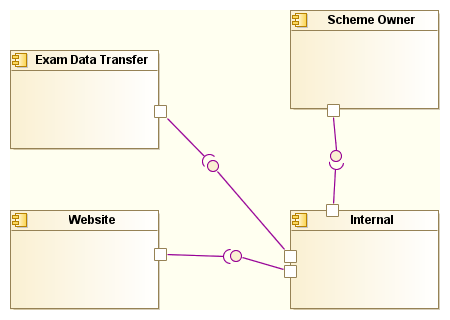
\includegraphics[scale=0.6]{uml/vision.png}
    \caption{Systemvision der Komponenten}
\end{figure}

Aufbauend darauf wurde dann versucht einen Prozess zu finden, der diese Grundideen berücksichtigt.

Die anfänglichen Versuche basierten stark auf einem ATAM Utility Tree ähnlichen Verfahren, bei welchem die nicht funktionalen Anforderungen nach der Formel von Oliver Vogel priorisiert wurden: \glqq Priorität = (Nutzen + Risiko + Wirkung) / 3\grqq \cite[S. 374]{softarch}. Die Bewertung der Komponenten wurde auf Basis einer bestehenden Tabelle mit Basisarchitekturen abgeleitet \cite[S. 179]{review}.


\subsection{Vom Usecase zur Komponente durch Priorisierung der nicht funktionalen Anforderungen}
Der erste Versuch zur Erstellung des Architekturprozesses orientierte sich am Prinzip: teile und herrsche. Der Prozess verwendete aufgrund der initialen Vermutung, dass nicht funktionalen Anforderungen die Hauptentscheidungsbasis für die Architektur darstellen, eine priorisierte Liste von nicht funktionalen Anforderungen. Danach wurde versuchte, anhand der priorisierten Anforderungen passende Komponenten auszuwählen. Der Ablauf war folgender:

\begin{itemize}
  \item Für jeden Usecase wird ein komplettes Komponentendiagramm des Systems erstellt.
  \item Die Komponenten jedes Teilsystems werden anhand ihrer nicht funktionalen Qualitäten aus einem Pool von Komponentenarchitekturen gewählt. Diese Komponentenarchitekturen beinhalteten zB. Systeme wie den üblichen Webstack, welcher sich aus Komponenten wie dem Loadbalancer, Datenbankserver, Applikationsserver und Webserver zusammensetzt.
  \item Schlussendlich werden alle Teilsysteme miteinander vereinigt, soweit es die nicht funktionalen Attribute erlauben.
\end{itemize}

Dieser Prozess scheiterte nicht nur am enormen Modellierungsaufwand, sondern auch am Auswahlprozess der Komponentenarchitekturen: Je nachdem, welche Komponentenarchitekturen vorhanden waren und wie diese bewertet wurden, entstanden unterschiedliche Architekturen. Zudem schien es zu viele Komponentenarchitekturen zu geben, da einzelnen Komponenten beliebig miteinander kombinierbar waren.

Die Qualität der Architektur hätte folglich von der Vollständigkeit dieser scheinbar unendlich großen Menge an Komponentenarchitekturen abgehangen. Aus diesem Grund schien der Prozess ungeeignet für die Architekturerstellung und wurde somit verworfen.

\subsection{Von einer Architektur mit hoher Kohäsion und anschließendem Architekturreview zu den Komponenten}
Um das Problem des sehr hohen Modellierungsaufwandes des ersten Prozesses zu umgehen, wurde von einer Grundarchitektur mit hoher Kohäsion ausgegangen. Diese Komponentenarchitektur entstand zusammen mit dem/der AuftraggeberIn, um zusätzliche Risiken indentifizieren zu können.

\begin{figure}[!htbp]
    \centering
    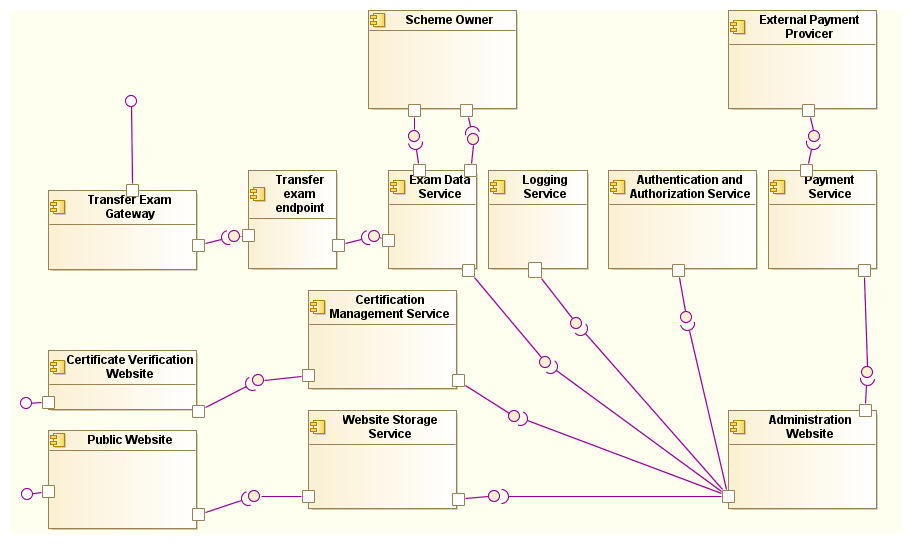
\includegraphics[scale=0.5]{uml/vision2.png}
    \caption{Architektur mit hoher Kohäsion}
\end{figure}

Diese Architektur sollte nun auf die Erfüllung der nicht funktionalen Anforderungen überprüft und gegebenenfalls angepasst werden. Zur Überprüfung der Anforderungen wurden die priorisierten, nicht funktionalen Anforderungen eines Usecases herangezogen. Der Prozess ähnelte damit stark einem szenariobasierten Review wie er in ATAM durchgeführt wird.

Auch dieser Prozess litt jedoch unter dem Problem, dass die nicht funktionalen Anforderungen schwer bewertet werden konnten. Außerdem war es schwer ein Regelwerk/Rezept aus der Architekturerstellung abzuleiten, da durch die Einbeziehung unterschiedlicher AuftraggeberInnen jeweils verschiedene Architekturen entstehen können. Die Einbeziehung von Kohäsion als Aufteilungsgrundlage der Komponenten verursachte zudem ein gefühlt zu großes System, welches in der Umsetzung sehr teuer geworden wäre. Die Kostenersparnis des Systems, welche in der Systemvision definiert wurde, schien damit unzureichend erfüllt zu werden.

\subsection{Von den Daten zu den Komponenten}
Die Auswahl und Bewertung der Komponentenarchitekturen und der starke Fokus auf die nicht funktionalen Anforderungen in den beiden vorherigen Prozessen stellte ein wesentliches Hindernis zur Erstellung eines eindeutigen Regelwerkes dar: Eine vollständige Auflistung aller möglichen Komponentenarchitekturen erschien entweder unmöglich oder unvollständig zu sein; eine Bewertung der nicht funktionalen Attribute schien ohne entsprechende Implementation nur sehr grob überprüfbar zu sein. Der Versuch, ein System mit hoher Kohäsion zu erstellen, endete zudem in sehr teuren Architekturen.

Dies war überraschend, da die populärste Architekturbewertungsmethode, ATAM, stark auf nicht funktionale Anforderungen aufbaute. Als Grund für diese Inkompatibilität wurde der Zeitpunkt der Architekturerstellung vermutet: Durch die fehlende Implementationsphase waren die nicht funktionalen Anforderungen sehr schwer zu bewerten und somit mehr oder weniger nicht überprüfbar. Deshalb wurden sie als Hauptkriterium und Ausgangspunkt für die Architekturerstellung verworfen.

Stattdessen wurde der Fokus auf die Aufspaltung der Daten gelegt. Die Daten wurden anhand Ihrer Vertraulichkeit in unterschiedliche Netze aufgeteilt. Diese Netze wurden dann durch Komponenten miteinander verbunden, die den Zugriff auf die Daten regelten.

\begin{figure}[!htbp]
    \centering
    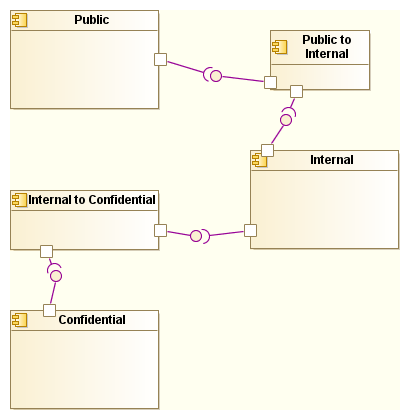
\includegraphics[scale=0.7]{uml/vision3.png}
    \caption{Aufteilung der Komponenten in Datenbereiche}
\end{figure}

Dieser Prozess erlaubte es, eine nachvollziehbare Architektur zu erstellen, jedoch war das Ergebnis zu grob. Außerdem schien eine separate Komponente zur  Übertragung der Prüfungsdaten zu fehlen, welche in der ursprünglichen Systemvision definiert und als notwendig empfunden worden war, um die Rahmenbedingungen der Vertrautheit zu erfüllen \cite[7.3]{ISO_CERT}.

\subsection{Von den Daten und den AkteurInnen zu den Komponenten}
Aufbauend auf dem vorherigen Prozess, welcher die Architektur anhand der Daten erstellte, wurden nun auch AkteurInnen eingebunden und deren Beziehungen zu den Daten ermittelt. Anhand dieser Beziehungen wurden Regeln erstellt, aus denen wiederum die Architektur erstellt wurde.

\begin{figure}[!htbp]
    \centering
    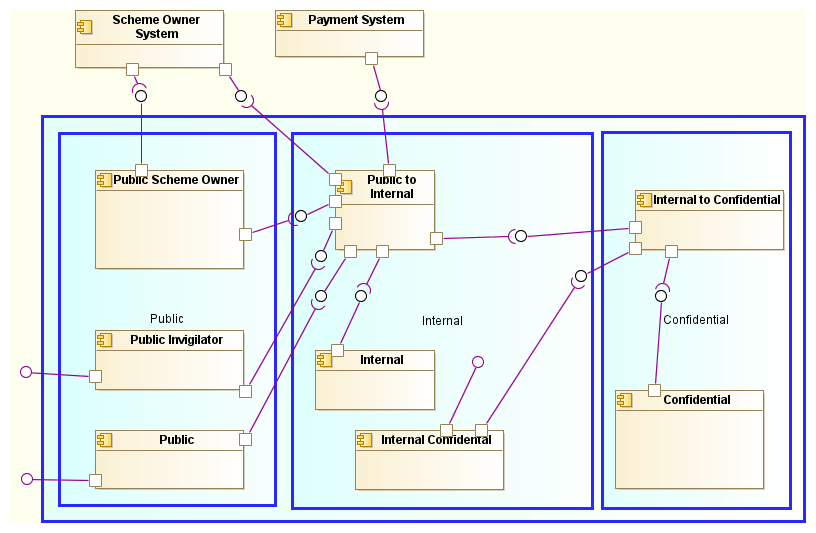
\includegraphics[scale=0.55]{uml/vision4.png}
    \caption{Aufteilung der Komponenten in Datenbereiche und AkteurInnen}
\end{figure}

Dieser Prozess schien nicht nur die Rahmenbedingungen und Sicherheitsbedingungen abzudecken, er war auch durch die erstellten Regeln nachvollziehbar und genau genug, um bereits einen guten Überblick auf die Architektur zu erlangen. Anhand der daraus resultierenden Architektur war es nun auch möglich, nicht funktionale Attribute wie zB. Antwortzeiten besser einschätzen zu können.


\chapter{Prozess Anforderungen}
Wie wurde der Anforderungsprozess angepasst und durchgeführt? Vermutung gute Architektur hängt von nicht funktionalen Anforderungen ab treibender Faktor

\section{Modellierung der Usecases}
Usecase diagramm

\section{Überführen der Usecases in Anforderungstemplate}
Warum wurde ein Template und welches wurde verwendet

\section{Anpassen des Anforderungstemplates}
Welche Sachen konnten schon vorher ermittelt werden
\subsection{Wachstumsszenarien und Wahrscheinlichkeit}
\subsection{Änderungsszenarien}
\subsection{Businesskritikalität}
Ausfallkosten, Datenverlustszenarien
\subsection{Rahmenbedingungen}

\section{Modellierung der Daten}
Klassendiagramm der Daten

\section{Modellierung der Akteure und Partnersysteme}
Kontextdiagramm der Akteure und Systeme


\chapter{Prozess Architekturplanung}
\section{Erstellen der Minimalen Architektur}
Ausgehen vom Kontextdiagramm

\section{Datenaufteilung nach Vertrautheitslevel}
Erweitern der Daten mit eigenen Stereotypen,

\section{Akteuraufteilung nach Vertrautheitslevel}
Erweitern der Akteure mit eigenen Stereotypen

Modellierung der Daten x Akteure (CRUD Matrix), Erklären dass man mit Aktivitätsdiagramm auf Matrix kommt

\section{Erstellen der Datenminimalarchitektur}
Einteilen der Systeme in Vertrautheitslevel und mit Gateways trennen. Datenflüsse fix vorgeben (darf keinen Gateway überspringen). Erklären was die Gateways machen und warum sie gut skalierien

\section{Einbeziehen der Akteure}
Trennen von Akteursystemen basierend auf Daten und Vertrautheitslevel

\section{Modellieren der Komponenten Interfaces (Klassen Diagramm)}
Aufzeigen dass zb das interne System user anlegen können muss mit methoden im klassendiagramm

\section{Analyse der nicht funktionalen Attribute}
Auf Basis von dokumentierten Szenarien können nun nicht funktionale Attribute gemessen werden und Hinweise kritische/wichtige Komponenten gegeben werden. Kostengegenüberstellung können auch eigene Systeme rechtfertigen/entfernen

\subsection{Reliability}
Single Point of Failure Analyse (Matrix Komponente x Usecase), Erklären wie man auf Matrix kommt (Aktivitätsdiagramm), Ausfallskosten (inkl. Wachstumsszenarien)

Einfache Methode zur schätzung der Ausfallkosten, aufzeigen wie durch Reduzieren der Ausfallswahrscheinlichkeit Kosten sinken aber auch Investitionskosten verursachen. Wachstumsszenarien auch einbeziehen in die Rechnung
\subsection{Usability}
In diesem Teil des Prozesses nicht wichtig, da noch keine Implementierung vorhanden.

\subsection{Efficiency}
Efficiency kann pro usecase gemessen werden, zb für antwortzeiten indem man zb die swimlanewechsel der Aktivitätsdiagramme zählt und mit einer konstanten multipliziert (geschätzte Netzwerkgeschwindigkeit). Ansonsten ist es durch die fehlende Implementation nicht möglich die Geschwindigkeit oder den Arbeitsspeicherverbrauch zu messen.

\subsection{Maintainability}
Auslesbar aus der Usecase Matrix, als Summe aller subsysteme,

\subsection{Portability}
In diesem Teil des Prozesses nicht wichtig, da noch keine Implementierung vorhanden.

\section{Changemanagement}
Je nachdem ob noch möglich/gewünscht aufzeigen wie würde ein Change request ausschauen, z.B. was wäre nötig um einen zusätlichen Typ User des Systems einzubinden


\chapter{Zusammenfassung}

\section{Warum ist der Prozess gut}
\subsection{10er Regel der Fehlerkosten}
\subsection{Lässt Entscheidungen aufschieben}
\subsection{Kochrezept lässt sich ableiten}
\subsection{Wichtige Anforderungsparameter schon früh einbezogen}
\subsection{Visuelle Repräsentationen mit denen schnell bewertet werden kann}

\section{Limitierungen}
\subsection{Nicht alle nicht funktionalen Anforderungen überprüfbar}
Sprich es ist bis zu einem gewissen Teil möglich
\subsection{Problem wenn sicht Akteure/Daten oft ändern}
\subsection{Zum Teil auch abhängig von Erfahrungswerten}
\subsection{Nur Plangungsphase, ohne Implementierungsphase}
\subsection{Extremarchitekturen}

\section{Erkenntnisse}
\subsection{Ohne messbare Parameter kein Kochrezept möglich}
\subsection{Parameter nicht zu jeder Phase messbar}
\subsection{Priorisierung von nicht funktionalen Parametern schwer möglich}
\subsection{Generische Komponentenarchitektur durch viele und schnell ändernde Kombinationen schwer möglich}
\subsection{Auf Ehrfahrungswerte kann nicht vollkommen verzichtet werden}
\subsection{Funktionale Anforderungen beeinflussen Archtitektur mehr als gedacht}
Prozess erstellt die frühe Architektur hauptsächlich durch einbeziehen funktionaler parameter, nicht funktionale parameter wegen fehlender implementation schwer messbar.

\section{Ausblick}
Prozess in der Planungsphase erprobt. Implementierungsphase auch wichtig, aber nicht beschrieben. Nächste Schritte könnten sein den Prozess mit einer Implementierungsphase zu erweitern. 1 Projekt hat viele Probleme schon aufgezeigt, aber weitere, unterschiedliche Projekte wären gut um den Prozess noch zu verbessern.

\clearpage
\bibliographystyle{gerabbrv}
\bibliography{Literatur}
\clearpage

% Das Abbildungsverzeichnis
\listoffigures
\clearpage

% Das Tabellenverzeichnis
\listoftables
\clearpage

% Das Quellcodeverzeichnis
\listofcode
\clearpage

\phantomsection
\addcontentsline{toc}{chapter}{Abkürzungsverzeichnis}
\chapter*{Abkürzungsverzeichnis}
\begin{acronym}[XXXXX]
    \acro{VPN}[VPN]{Virtual Private Network}
    \acro{WWW}[WWW]{world wide web}
\end{acronym}
\clearpage

\phantomsection
\addcontentsline{toc}{chapter}{Anhang}
\chapter*{Anhang}


\end{document}
